\chapter{Трансформеры на практике}
\label{chap:transformers_in_practice}

\begin{supportbox}{Об этой главе}
Теперь мы рассмотрим несколько вариаций базовой модели трансформера, включая архитектуры кодер-декодер, причинные слои MHA и приложения к областям изображений и аудио.
\end{supportbox}

\section{Трансформеры кодер-декодер}

Модель, которую мы описали в Главе \ref{chap:transformers}, может использоваться для выполнения регрессии или классификации заданной последовательности. Однако оригинальный трансформер \cite{vaswani2017attention} был более сложной моделью, разработанной для так называемых \textbf{последовательность-в-последовательность} (seq2seq) задач. В задаче seq2seq и вход, и выход являются последовательностями, и между их токенами нет тривиального соответствия. Ярким примером является \textbf{машинный перевод}, в котором выход является переводом входной последовательности на другой язык.

Одна из возможностей построения дифференцируемой модели для задач seq2seq — это дизайн \textbf{кодер-декодер} (ED) \cite{sutskever2014sequence}. Модель ED состоит из двух блоков: кодера, который обрабатывает входную последовательность в преобразованное представление (возможно, фиксированной размерности), и декодера, который авторегрессионно генерирует выходную последовательность, обусловленную выходом кодера. Модель трансформера, которую мы описали ранее, может использоваться для построения кодера: трансформеры этого типа для классификации называются \textbf{только-кодерными} трансформерами. Чтобы построить декодер, нам нужны два дополнительных компонента: способ сделать модель причинной (для выполнения авторегрессии) и способ обусловить ее вычисление отдельным входом (выходом кодера).

\subsection{Причинное многоголовочное внимание} \addclock

Давайте сначала рассмотрим проблему создания причинного блока трансформера. Единственный компонент, в котором взаимодействуют токены, — это блок MHA. Следовательно, наличие причинного варианта MHA достаточно, чтобы сделать всю модель причинной. Помните, что для свёрток мы разработали причинный вариант, соответствующим образом маскируя веса в свёрточном фильтре. Для MHA мы можем вместо этого маскировать все взаимодействия между токенами, которые не удовлетворяют свойству причинности:
%
$$
\text{Masked-SA}(\mathbf{X})=\text{softmax}\left(\frac{\mathbf{Q}\mathbf{K}^\top {\color{drawred_l}\odot \,\mathbf{M}}}{\sqrt{k}}\right)\mathbf{V}
$$
%
Важно выполнять маскирование внутри softmax. Рассмотрим следующий (неправильный) вариант:
%
$$
\text{\color{red}\textbf{Неправильно}:} \;\;\left(\text{softmax}\left(\frac{\mathbf{Q}\mathbf{K}^\top }{\sqrt{k}}\right){\color{drawred_l}\odot \,\mathbf{M}}\right)\mathbf{V}
$$
%
Из-за знаменателя в softmax все токены участвуют в вычислении каждого токена, независимо от последующего маскирования. Также обратите внимание, что установка $M_{ij}=0$ для непричинных связей не работает, потому что $\exp(0)=1$. Следовательно, правильная реализация замаскированного варианта MHA заключается в выборе верхнетреугольной матрицы с $-\infty$ в верхней части, поскольку $\exp(-\infty)=0$, как и требовалось:
%
$$
M_{ij} =\begin{cases} -\infty & \text{ если } i > j \\ 0 & \text{ иначе } \end{cases}
$$
%
Практически, значения можно установить на очень большое отрицательное число (например, $-10^9$).

\begin{SCfigure}
    \centering
    \hspace{1em}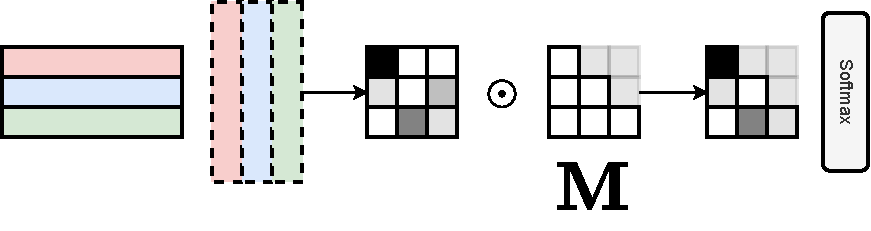
\includegraphics[width=0.7\textwidth]{images/attention_masked}
    \caption{Визуальное изображение причинного внимания, реализованного с помощью маскирования внимания.}
    \label{fig:masked_attention}
\end{SCfigure}

\subsection{Перекрестное внимание}

Во-вторых, давайте рассмотрим проблему зависимости выхода слоя MHA от отдельного блока входов. Для этого перепишем операцию MHA, явно разделив три появления входной матрицы:
%
$$
\text{SA}({\color{drawred}\mathbf{X}_1}, {\color{drawgreen}\mathbf{X}_2}, {\color{drawblue}\mathbf{X}_3})=\text{softmax}\left(\frac{{\color{drawred}\mathbf{X}_1}\mathbf{W}_q\mathbf{W}_k^\top{\color{drawgreen}\mathbf{X}_2^\top}}{\sqrt{k}}\right){\color{drawblue}\mathbf{X}_3}\mathbf{W}_v
$$
%
Слой SA соответствует $\mathbf{X}_1 = \mathbf{X}_2 = \mathbf{X}_3 = \mathbf{X}$ (что, по совпадению, объясняет данное ему название). Однако формулировка также работает, если мы рассматриваем ключи, значения и запросы, принадлежащие разным множествам. Одним из важных случаев является \textbf{перекрестное внимание} (CA), в котором мы предполагаем, что ключи и значения вычисляются из второй матрицы $\mathbf{Z} \sim (m,e)$:

\begin{equation}
\text{CA}(\mathbf{X}, \mathbf{Z}) = \text{SA}(\mathbf{X}, \mathbf{Z}, \mathbf{Z}) = \text{softmax}\left(\frac{\eqnmarkbox[drawred]{node}{\mathbf{X}\mathbf{W}_q\mathbf{W}_k^\top\mathbf{Z}^\top}}{\sqrt{k}}\right)\mathbf{Z}\mathbf{W}_v
\label{eq:ca}
\end{equation}
\annotate[yshift=1em]{above,right}{node}{Перекрестное внимание между $\mathbf{X}$ и $\mathbf{Z}$}

Интерпретация заключается в том, что вложения $\mathbf{X}$ обновляются на основе их сходства с набором внешних пар (ключ, значение), предоставляемых $\mathbf{Z}$: мы говорим, что $\mathbf{X}$ \textit{перекрестно-внимает} на $\mathbf{Z}$. Обратите внимание, что эта формулировка очень похожа на конкатенацию двух наборов входных токенов с последующим соответствующим маскированием матрицы внимания.

\subsection*{Сравнение с полносвязными слоями} \addteacup
\label{subsec:comparison_ca_mlp}

Рассмотрим упрощенный вариант операции перекрестного внимания в \eqref{eq:ca}, в котором мы явно параметризуем матрицы ключей и значений:\footnote{См. также обсуждение сети перцептрона в Разделе \ref{subsec:time_complexity_mha}.}
%
\begin{equation}
\text{NeuralMemory}(\mathbf{X}) = \text{softmax}\left(\frac{\mathbf{X}\mathbf{W}_q {\color{drawred}\mathbf{K}}}{\sqrt{k}}\right){\color{drawgreen}\mathbf{V}}
\label{eq:memory_layer}
\end{equation}
%
Слой теперь параметризован матрицей проекции запроса $\mathbf{W}_q$ и двумя матрицами ${\color{drawred}\mathbf{K}}$ и ${\color{drawgreen}\mathbf{V}}$. \eqref{eq:memory_layer} называется \textbf{слоем памяти} \cite{sukhbaatar2015end}, в том смысле, что строки матриц ключей и значений используются моделью для хранения интересных паттернов, которые динамически извлекаются с помощью операции, подобной вниманию. Если мы еще больше упростим слой, установив $\mathbf{W}_q = \mathbf{I}$, игнорируя нормализацию на $\sqrt{k}$ и заменяя softmax на общую функцию активации $\phi$, мы получим двухслойный МЛП:
%
\begin{equation}
\text{MLP}(\mathbf{X}) = \phi\left(\mathbf{X}\mathbf{K}\right)\mathbf{V}
\end{equation}
%
Следовательно, МЛП в сетях-трансформерах можно рассматривать как аппроксимацию операции внимания над обучаемыми ключами и значениями. Визуализация ближайших токенов в обучающих данных показывает понятные человеку паттерны \cite{geva2020transformer}.

\subsection{Полный трансформер кодер-декодер}

\begin{figure}[t]
    \centering
    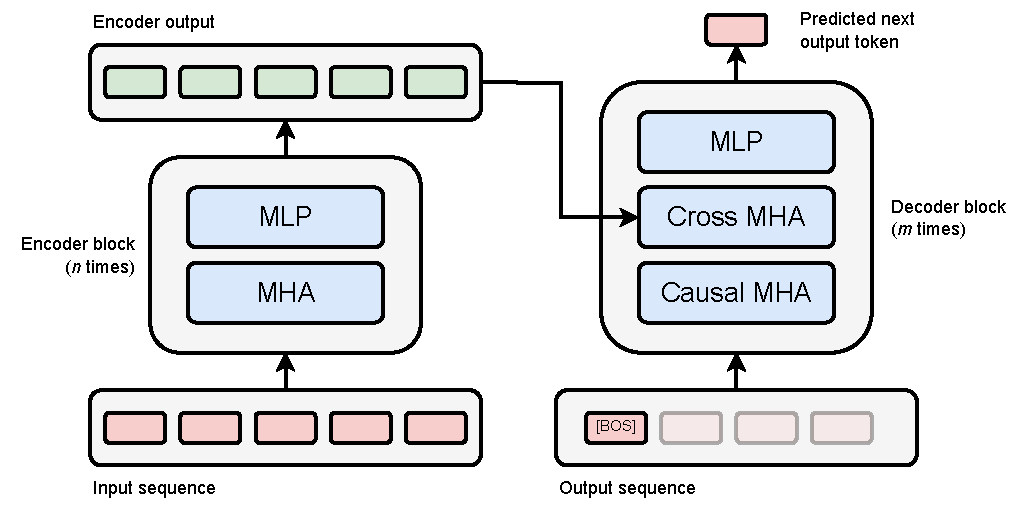
\includegraphics[width=0.8\textwidth]{images/transformer_architecture}
    \caption{Архитектура кодер-декодер, адаптированная из \cite{vaswani2017attention}. Дополненные токены в декодере затенены.}
    \label{fig:transformer_model}
\end{figure}

С этими двумя компонентами в руках мы готовы обсудить оригинальную модель трансформера, показанную на Рисунке \ref{fig:transformer_model}.\footnote{Педантичное примечание: технически, Transformer (с заглавной буквы) — это имя собственное в \cite{vaswani2017attention}. В книге я использую трансформер (со строчной буквы) для обозначения любой модели, состоящей в основном из слоев внимания.} Во-первых, входная последовательность $\mathbf{X}$ обрабатывается стандартной моделью трансформера (называемой \textbf{кодером}), предоставляя обновленную последовательность вложений $\mathbf{H}$. Затем выходная последовательность предсказывается авторегрессионно другой моделью трансформера (называемой \textbf{декодером}). В отличие от кодера, декодер имеет три компонента для каждого блока:
%
\begin{enumerate}
\item Замаскированный вариант слоя MHA (чтобы обеспечить возможность авторегрессии).
\item Слой перекрестного внимания, где запросы задаются вложением входной последовательности $\mathbf{H}$.
\item Стандартный токен-ориентированный МЛП.
\end{enumerate}
%
Также возможны модели \textbf{только-декодеры}, и в этом случае второй блок декодера удаляется, и используются только замаскированные MHA и МЛП. Большинство современных БЯМ построены на моделях только-декодерах, обученных авторегрессионно генерировать текстовые токены \cite{radford2019language}, как обсуждалось ниже. Фактически, модели кодер-декодер стали менее распространены с осознанием того, что многие задачи seq2seq можно решать непосредственно с помощью моделей только-декодеров, объединяя входную последовательность с генерируемой выходной последовательностью, как описано в Разделе \ref{subsec:conditional_modelling}.

\section{Вычислительные соображения}

\subsection{Временная сложность и линейно-временные трансформеры}
\label{subsec:time_complexity_mha}

Производительность MHA не обходится без затрат: поскольку каждый токен должен обращать внимание на все остальные токены, его сложность выше, чем у более простой свёрточной операции. Чтобы понять это, мы рассмотрим его сложность с двух точек зрения: памяти и времени. Мы используем наивную реализацию слоя SA для справки, показанную в Листинге \ref{code:sa}.

\begin{mypy}{Простая реализация слоя SA, явно параметризованная в терминах матриц запроса, ключа и значения.}{code:sa}
def self_attention(Q: Float[Array, "n k"], 
                   K: Float[Array, "n k"], 
                   V: Float[Array, "n v"]
                 ) -> Float[Array, "n v"]:
	return nn.softmax(Q @ K.T) @ V
\end{mypy}

Давайте сначала посмотрим на временную сложность. Операция внутри softmax масштабируется как $\mathcal{O}(n^2k)$, потому что ей нужно вычислить $n^2$ скалярных произведений (по одному для каждой пары токенов). Сравните это с 1D-свёрточным слоем, который масштабируется только линейно по длине последовательности. \textit{Теоретически}, этот квадратичный рост сложности может быть проблематичным для очень больших последовательностей, которые распространены, например, в БЯМ. 

Это привело к разработке нескольких стратегий для ускорения авторегрессионной генерации (например, спекулятивное декодирование \cite{leviathan2023fast}), а также линейных или субквадратичных вариантов трансформеров. В качестве примера, мы можем заменить слой SA на слой перекрестного внимания с \textit{обучаемым} набором токенов $\mathbf{Z}$, где количество токенов можно выбрать как гиперпараметр и контролировать пользователем. Эта стратегия была популяризирована архитектурой Perceiver \cite{jaegle2021perceiver} для дистилляции исходного набора токенов в меньшие скрытые узкие места. Существует много альтернативных стратегий для проектирования линеаризованных трансформеров: мы обсудим несколько вариантов в Разделе \ref{subsec:mha_variants} и Главе \ref{chap:rnns}.

Важно, что реализация, подобная той, что в Листинге \ref{code:sa}, может быть сильно ограничена памятью на современном оборудовании \cite{dao2022flashattention}, что означает, что ее вычислительная стоимость определяется операциями с памятью и вводом-выводом. Следовательно, теоретические выгоды от линейно-временных вариантов внимания не коррелируют с фактическим ускорением на оборудовании. В сочетании с возможным снижением производительности это делает их менее привлекательными, чем сильно оптимизированная реализация MHA, такая как описанная далее.

\subsection{Сложность по памяти и онлайн-softmax}

С точки зрения памяти, реализация в Листинге \ref{code:sa} также имеет квадратичный фактор сложности $n^2$, потому что матрица внимания $\mathbf{Q}\mathbf{K}^\top$ полностью материализуется во время вычисления. Однако это необязательно, и эту сложность можно значительно уменьшить до линейного фактора, разбив вычисление на блоки и выполняя нормализацию softmax только в конце \cite{rabe2021self}. 

Чтобы понять это, рассмотрим один вектор запроса $\mathbf{q}$ и предположим, что мы разбиваем наши ключи и значения на два блока, которые по очереди загружаются в память:

\begin{equation}
\mathbf{K} = \begin{bmatrix}\mathbf{K}_1 \\ \mathbf{K}_2 \end{bmatrix} \;\;\; \mathbf{V} = \begin{bmatrix}\mathbf{V}_1 \\ \mathbf{V}_2 \end{bmatrix}
\end{equation}

Если мы проигнорируем знаменатель в softmax, мы можем разложить операцию SA, вычисляя выход для каждого блока по очереди:

\begin{equation}
\text{SA}(\mathbf{q}, \mathbf{K}, \mathbf{V}) = \frac{1}{L_1 + L_2} \left[ \mathbf{h}_1 + \mathbf{h}_2 \right]
\label{eq:attention_two_chunks}
\end{equation}

где для двух блоков $i=1,2$ мы определили две вспомогательные величины:
%
\begin{gather}
\mathbf{h}_i = \exp\left( \mathbf{K}_i\mathbf{q} \right)\mathbf{V}_i  \\
L_i = \sum_j \idx{\exp\left( \mathbf{K}_i\mathbf{q} \right)}{j}
\end{gather}
%
Помните, что мы загружаем блоки в память по отдельности, следовательно, для блока $1$ мы вычисляем $\mathbf{h}_1$ и $L_1$; затем мы выгружаем предыдущий блок и вычисляем $\mathbf{h}_2$ и $L_2$ для блока 2. Обратите внимание, что операция не является полностью разложимой, если мы не отслеживаем дополнительные статистики $L_i$ (которые необходимы для вычисления коэффициентов нормализации операции softmax). В более общем случае, для нескольких блоков $i=1, \ldots, m$ мы будем иметь:

\begin{equation}
\text{SA}(\mathbf{q}, \mathbf{K}, \mathbf{V}) = \frac{1}{\sum_{i=1}^m L_i} \left[ \sum_{i=1}^m \mathbf{h}_i\right]
\label{eq:chunked_sa}
\end{equation}

Следовательно, мы можем разработать простой итерационный алгоритм, где для каждого блока ключей и значений, загруженных в память, мы обновляем и храним кумулятивную сумму числителя и знаменателя в \eqref{eq:chunked_sa}, выполняя нормализацию только в конце. Этот трюк (иногда называемый \textit{онлайн} softmax), в сочетании с IO-осведомленной реализацией и слиянием ядер, привел к высокоэффективным по памяти и вычислениям реализациям внимания, таким как FlashAttention-2.\footnote{\url{https://github.com/Dao-AILab/flash-attention}} Распределенные реализации внимания (например, RingAttention \cite{liu2023ring}) также могут быть разработаны путем назначения групп запросов разным устройствам и ротации блоков ключей и запросов между устройствами. Оптимизация операции для конкретного оборудования может привести к некоторым контринтуитивным поведениям, таким как \textit{увеличение} скорости при больших длинах последовательностей - см. Рисунок \ref{fig:flash_attention}.

\begin{figure}[t]
    \centering
    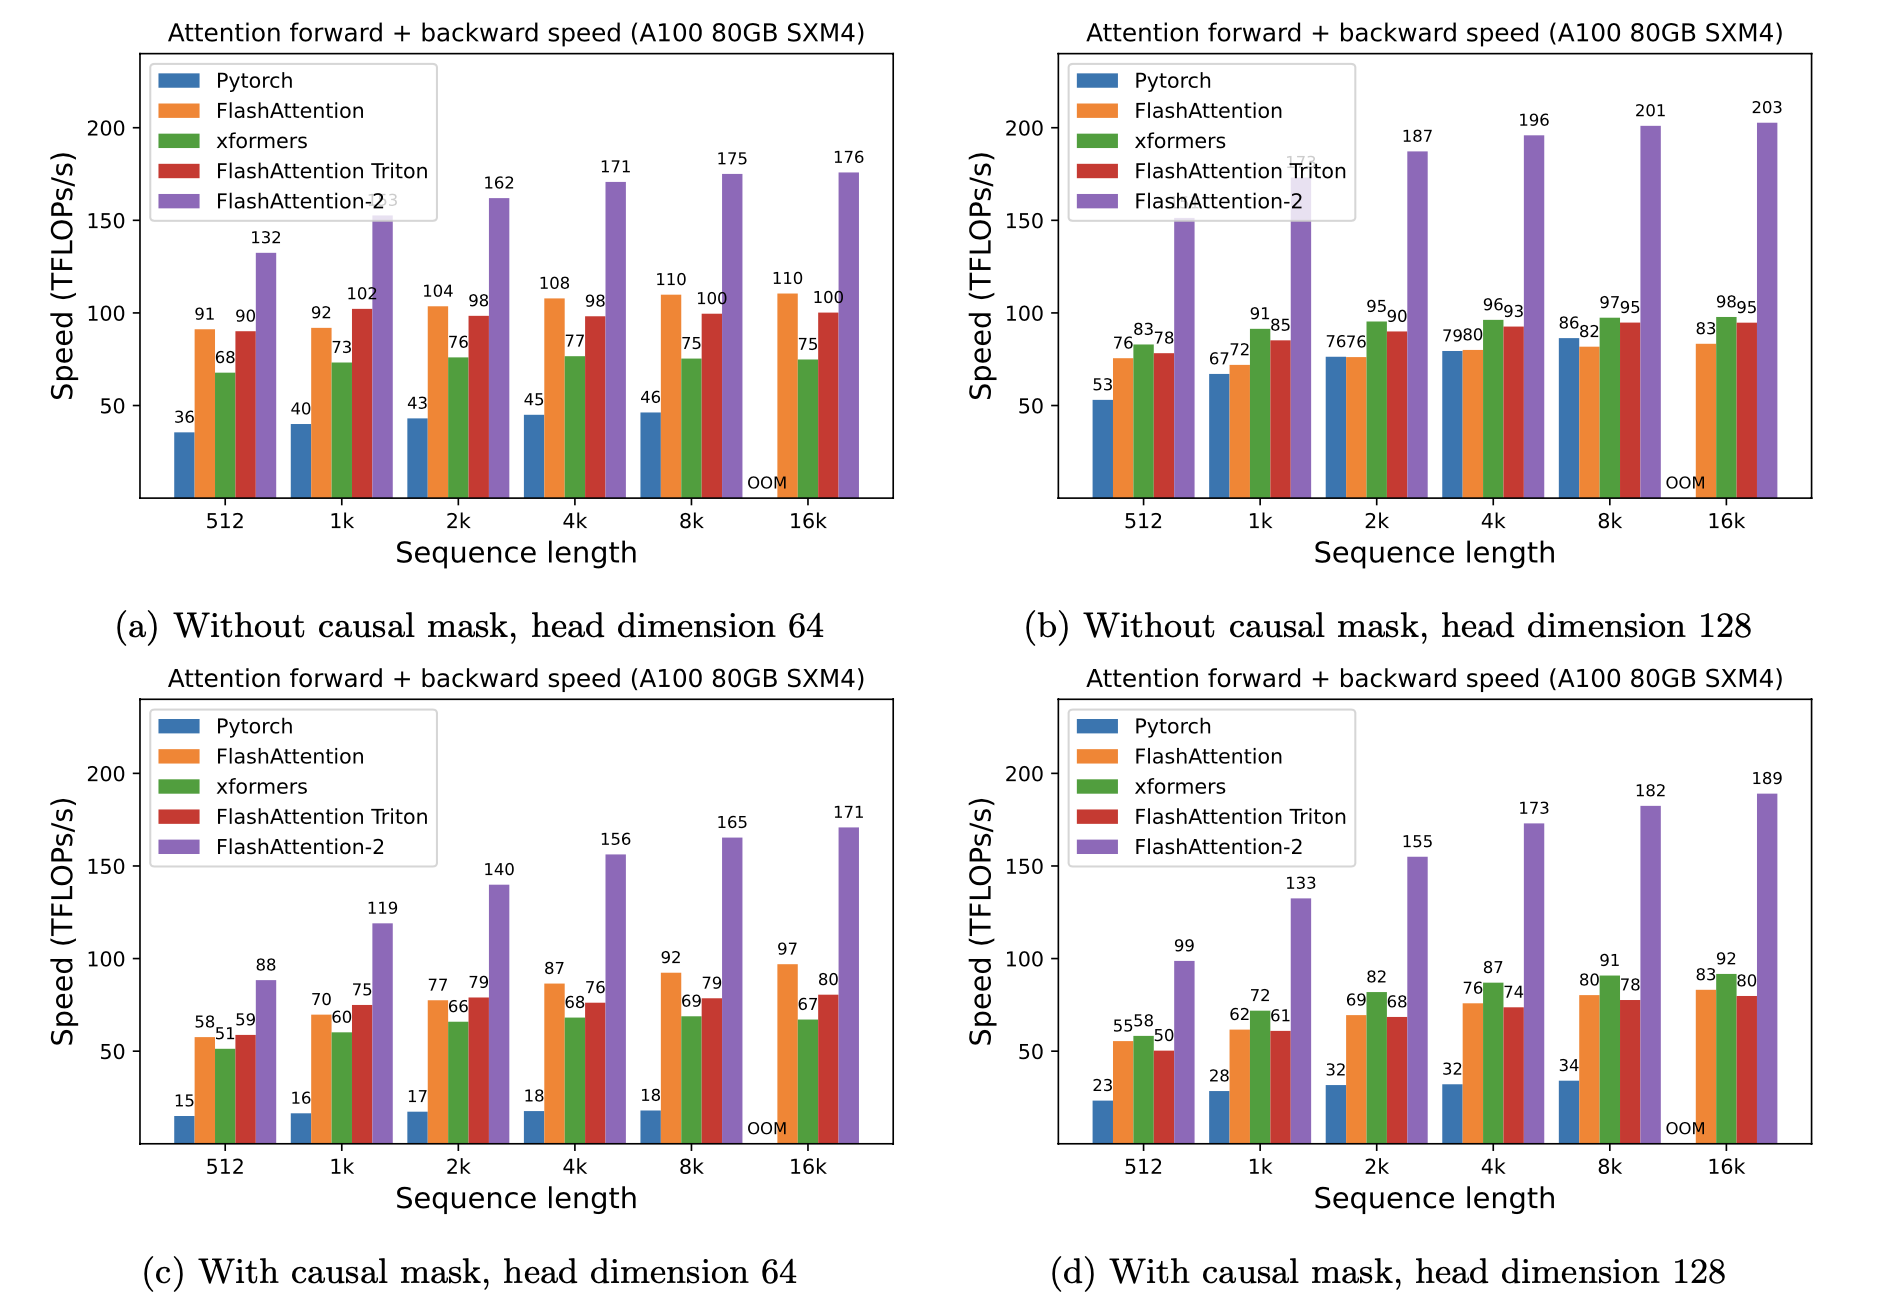
\includegraphics[width=0.7\textwidth]{images/flash2_a100_fwd_bwd_benchmark.png}
    \caption[Официальный бенчмарк FlashAttention и FlashAttention-2 на видеокарте NVIDIA A100.]{Официальный бенчмарк FlashAttention и FlashAttention-2 на видеокарте NVIDIA A100, воспроизведенный из \url{https://github.com/Dao-AILab/flash-attention}.}
    \label{fig:flash_attention}
\end{figure}

\subsection{Кэш KV}

Важный аспект реализации MHA возникает при работе с авторегрессионной генерацией в моделях только-декодерах. Для каждого нового генерируемого токена необходимо вычислить только новую строку матрицы внимания и один токен-значение, в то время как остальная часть матрицы внимания и оставшиеся токены-значения могут быть сохранены в памяти, как показано на Рисунке \ref{fig:kv_cache}. Это называется \textbf{кэшем KV} и является стандартом в большинстве оптимизированных реализаций MHA.

\begin{SCfigure}
    \centering
    \hspace{-0.5em}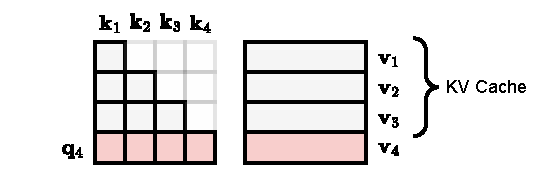
\includegraphics[width=0.6\textwidth]{images/kv_cache}
    \caption{Для вычисления замаскированного самовнимания для нового токена большую часть предыдущих вычислений можно повторно использовать (серым цветом). Это называется \textbf{кэшем KV}.}
    \label{fig:kv_cache}
\end{SCfigure}

Размер кэша KV линейно увеличивается с длиной последовательности. Еще раз, вы можете сравнить это с эквивалентной реализацией причинного свёрточного слоя, где память ограничена сверху размером рецептивного поля. Проектирование выразительных слоев с фиксированной стоимостью памяти при авторегрессионной генерации является мотивирующим фактором для Главы \ref{chap:rnns}.

\subsection{Трансформеры для изображений и аудио} \addteacup
\label{subsec:transformers_image_audio}

Трансформеры изначально были разработаны для текста и вскоре стали стандартным выбором для языкового моделирования. В частности, популярная модель GPT-2 \cite{radford2019language} (и более поздние варианты) — это архитектура только-декодера, которая предварительно обучается путем прогнозирования токенов в текстовых последовательностях. Большинство БЯМ с открытым исходным кодом, такие как LLaMa \cite{touvron2023llama}, следуют аналогичной архитектуре. Напротив, BERT \cite{devlin2018bert} — это другое популярное семейство предварительно обученных вложений слов, основанное на архитектуре только-кодера, обученной предсказывать замаскированные токены (\textbf{моделирование замаскированного языка}). В отличие от моделей типа GPT, модели типа BERT нельзя использовать для генерации текста, а только для выполнения вложения текста или в качестве первой части дообученной архитектуры. Также существуют модели кодер-декодер для языкового моделирования (например, семейство T5 \cite{raffel2020exploring}), но они стали менее популярными.

С высоты птичьего полета, трансформер состоит из трех компонентов: этапа токенизации/вложения, который преобразует исходный вход в последовательность векторов; позиционных вложений для кодирования информации о порядке исходной последовательности; и самих блоков трансформера. Следовательно, трансформеры для других типов данных можно спроектировать, определив соответствующую процедуру токенизации и позиционные вложения.

Давайте сначала рассмотрим компьютерное зрение. Токенизация изображения на уровне пикселей слишком дорога из-за квадратичного роста сложности по отношению к длине последовательности. Основная идея Vision Transformers (ViT, \cite{dosovitskiy2020image}) заключается в том, чтобы разделить исходный вход на непересекающиеся \textbf{патчи} фиксированной длины, которые затем сплющиваются и проецируются во вложение заранее определенного размера, как показано на Рисунке \ref{fig:image_tokenization}.

\begin{figure}[t]
    \centering
    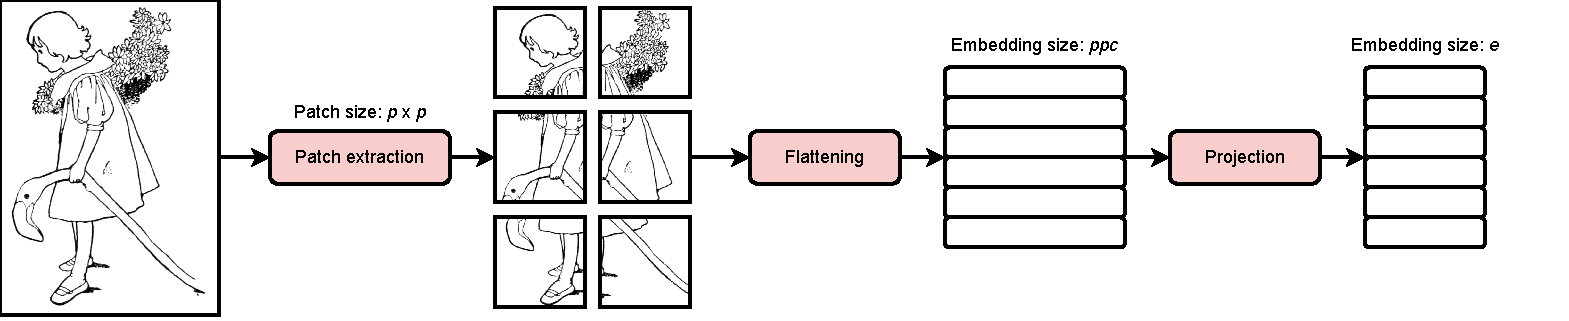
\includegraphics[width=1.0\textwidth]{images/image_tokenization}
    \caption{Токенизация изображения: изображение делится на непересекающиеся патчи формы $p \times p$ (где $p$ — гиперпараметр). Затем каждый патч сплющивается и подвергается дальнейшей линейной проекции в заданный пользователем размер вложения $e$. $c$ — количество каналов входного изображения.}
    \label{fig:image_tokenization}
\end{figure}

Этап вложения на Рисунке \ref{fig:image_tokenization} можно достичь с помощью свёрточного слоя с шагом, равным размеру ядра. В качестве альтернативы, библиотеки, такие как einops\footnote{\url{http://einops.rocks}}, расширяют операцию einsum (Раздел \ref{sec:linear_algebra}), чтобы разрешить группировку элементов в блоки заранее определенной формы. Пример показан в Листинге \ref{code:einops}.

Оригинальный ViT использовал обучаемые позиционные вложения вместе с дополнительным классовым токеном для выполнения классификации изображений. ViT также можно использовать для генерации изображений, предсказывая патчи в порядке строк или столбцов. В этом случае мы можем обучить отдельный модуль, который преобразует каждый патч в дискретный набор токенов используя, например, \textbf{векторно-квантованный вариационный автоэнкодер} \cite{chang2022maskgit}, или мы можем работать непосредственно с непрерывными выходами \cite{tschannen2023givt}. Однако для генерации изображений предпочтительны другие неавторегрессионные подходы, такие как диффузионные модели и согласование потоков; мы рассмотрим их в следующем томе.


\begin{mypy}{einops можно использовать для разложения изображения на патчи с помощью простого расширения синтаксиса einsum.}{code:einops}
def self_attention(Q: Float[Array, "n k"], 
                   K: Float[Array, "n k"], 
                   V: Float[Array, "n v"]
                 ) -> Float[Array, "n v"]:
	return nn.softmax(Q @ K.T) @ V
\end{mypy}

Разработав правильные механизмы токенизации и позиционные вложения, трансформеры также были разработаны для аудио, в частности для распознавания речи. В этом случае обычно используется небольшая 1D-свёрточная модель (с пулингом) в качестве блока токенизации \cite{baevski2020wav2vec,radford2023robust}. Например, Wav2Vec \cite{baevski2020wav2vec} — это модель только-кодера, выход которой обучается с расширением кросс-энтропийной потери, называемой потерей \textbf{коннекционистской временной классификации} \cite{graves2012connectionction}, для выравнивания выходных вложений с транскрипцией. Поскольку размеченных данных с точными выравниваниями мало, модели Wav2Vec предварительно обучаются на больших объемах неразмеченного аудио с вариантом потери моделирования замаскированного языка. Напротив, Whisper \cite{radford2023robust} — это модель кодер-декодер, где декодер обучается авторегрессионно генерировать транскрипцию. Это обеспечивает большую гибкость модели и снижает потребность в сильно размеченных данных, но за счет возможных \textit{галлюцинаций} на этапе транскрипции. Также можно обучать \textbf{нейронные аудиокодеки} для сжатия аудио в последовательность дискретных токенов \cite{defossez2022high}, которые, в свою очередь, составляют основу для генеративных приложений, таких как генерация речи из текста \cite{wang2023neural}.

Трансформеры также можно определить для временных рядов \cite{ansari2024chronos}, графов (рассматриваемых в следующей главе) и других типов данных. Разделение между данными и архитектурой также является основой для \textbf{мультимодальных} вариантов, которые могут принимать на вход (или предоставлять на выход) различные типы данных. Это достигается путем токенизации каждой модальности (изображение, аудио, ...) с помощью соответствующего токенизатора и объединения различных токенов в одну последовательность \cite{bordes2024introduction}. Мы показываем пример для \textbf{изображенческо-текстовой} модели на Рисунке \ref{fig:multimodal_transformer}.

\begin{SCfigure}
    \centering
    \hspace{1em}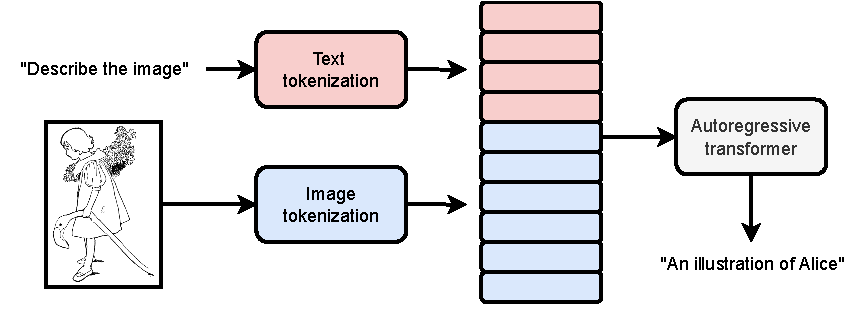
\includegraphics[width=0.65\textwidth]{images/multimodal_transformer}
    \caption{Пример \textbf{бимодального} трансформера, который работает как с изображениями, так и с текстом: выходы двух токенизаторов объединяются и отправляются в модель.}
    \label{fig:multimodal_transformer}
\end{SCfigure}

\section{Варианты блока трансформера}
\label{subsec:mha_variants}

Мы завершаем главу, обсуждая несколько интересных вариаций базового блока трансформера. Во-первых, было разработано несколько вариантов для очень больших трансформеров, чтобы немного сократить время вычислений или количество параметров. В качестве примера, \textbf{параллельные блоки} \cite{dehghani2023scaling} выполняют операции MLP и MHA параллельно:
%
$$
\mathbf{H} = \mathbf{H}+\text{MLP}(\mathbf{H})+\text{MHA}(\mathbf{H})
$$
%
Таким образом, начальные и конечные линейные проекции в слоях MLP и MHA могут быть объединены для более эффективной реализации. В качестве другого примера, \textbf{многозапросное MHA} \cite{shazeer2019fast} разделяет одну и ту же матрицу проекции ключа и значения для каждой головы, изменяя только запросы.

В более общем смысле, мы можем заменить слой MHA более простой (линейной по сложности по длине последовательности) операцией, сохраняя при этом общую структуру блока трансформера, т.е. чередуя смешивание токенов и каналов с послойной нормализацией и остаточными соединениями. В качестве примера, предположим, что длина последовательности фиксирована (например, для компьютерного зрения количество патчей можно зафиксировать априори). В этом случае слой MHA можно заменить на MLP, работающий с одним входным каналом, соответствующим одному измерению вложения. Этот тип модели называется моделью \textbf{микшера} \cite{tolstikhin2021mlp} - см. Рисунок \ref{fig:mlp_mixer}.
Игнорируя операции нормализации, это можно записать как чередующиеся МЛП на транспонированных версиях входной матрицы:
%
\begin{gather}
\mathbf{H}=\text{MLP}(\mathbf{H})+\mathbf{H} \\
\mathbf{H}= \left[\text{MLP}(\mathbf{H}^\top)+\mathbf{H}^\top\right]^\top
\end{gather}
%
Возможны и другие варианты модели микшера, использующие, например, 1D-свёртки, преобразования Фурье или пулинг. В частности, в модели S2-MLP \cite{yu2022s2} операция смешивания токенов заменяется еще более простым МЛП, применяемым к сдвинутой версии своего входа. Общий класс таких моделей был назван \textbf{MetaFormers} в \cite{yu2022metaformer}.

\begin{SCfigure}
    \centering
    \hspace{1em}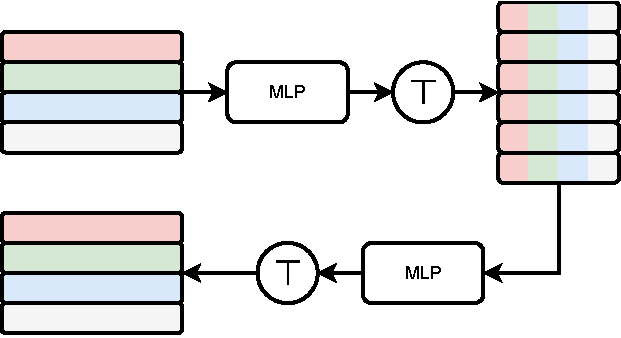
\includegraphics[width=0.55\textwidth]{images/mixer}
    \caption{Блок микшера, состоящий из чередующихся МЛП на строках и столбцах входной матрицы.}
    \label{fig:mlp_mixer}
\end{SCfigure}

Вентильные (мультипликативные) взаимодействия также могут использоваться в композиции блока. В этом случае несколько блоков выполняются параллельно, но их выход комбинируется с помощью произведения Адамара. Мы можем записать общий вентильный блок как:
%
\begin{equation}
f(\mathbf{X}) =\phi_1(\mathbf{X})\odot \phi_2(\mathbf{X})
\label{eq:glu_again}
\end{equation}
%
где $\phi_1$ и $\phi_2$ — обучаемые блоки. Например, с $\phi_1(\mathbf{X}) = \sigma(\mathbf{X}\mathbf{A})$ и $\phi_2(\mathbf{X})=\mathbf{X}\mathbf{B}$ мы получаем \textbf{вентильный линейный блок} (GLU), описанный в Разделе \ref{sec:activation_functions}.

В качестве нескольких характерных примеров, модель \textbf{gMLP} \cite{liu2021pay} использует
вентильные блоки вместо блока смешивания каналов в модели микшера; семейство моделей \textbf{LLaMa} \cite{touvron2023llama} использует блоки, подобные GLU, вместо стандартного блока MLP; в то время как \textbf{вентильный блок внимания} (GAU) \cite{hua2022transformer} использует более простую модель, подобную вниманию, с одной головой для $\phi_1$ и линейной проекцией для $\phi_2$. Эти дизайны особенно популярны в некоторых недавних вариантах рекуррентных моделей, обсуждаемых позже в Главе \ref{chap:rnns}.

Чтобы еще больше упростить дизайн, сеть мультилинейных операторов (MONet) удаляет все функции активации, чтобы определить блок, состоящий только из линейных проекций и поэлементных умножений \cite{cheng2024multilinear}:
%
$$
\mathbf{H}=\mathbf{E}(\mathbf{A}\mathbf{X}\odot\mathbf{B}\mathbf{X}+\mathbf{D}\mathbf{X})
$$
%
где $\mathbf{E}$ аналогично выходной проекции в блоке трансформера, $\mathbf{D}\mathbf{X}$ действует как остаточное соединение, а $\mathbf{B}$ реализуется с помощью низкорангового разложения для уменьшения количества параметров \cite{cheng2024multilinear}. Чтобы ввести смешивание токенов, во всех нечетных блоках модели реализована операция сдвига токенов.

\newpage
\section*{От теории к практике}

\begin{wrapfigure}{r}{3.0cm}
\vspace{-6em}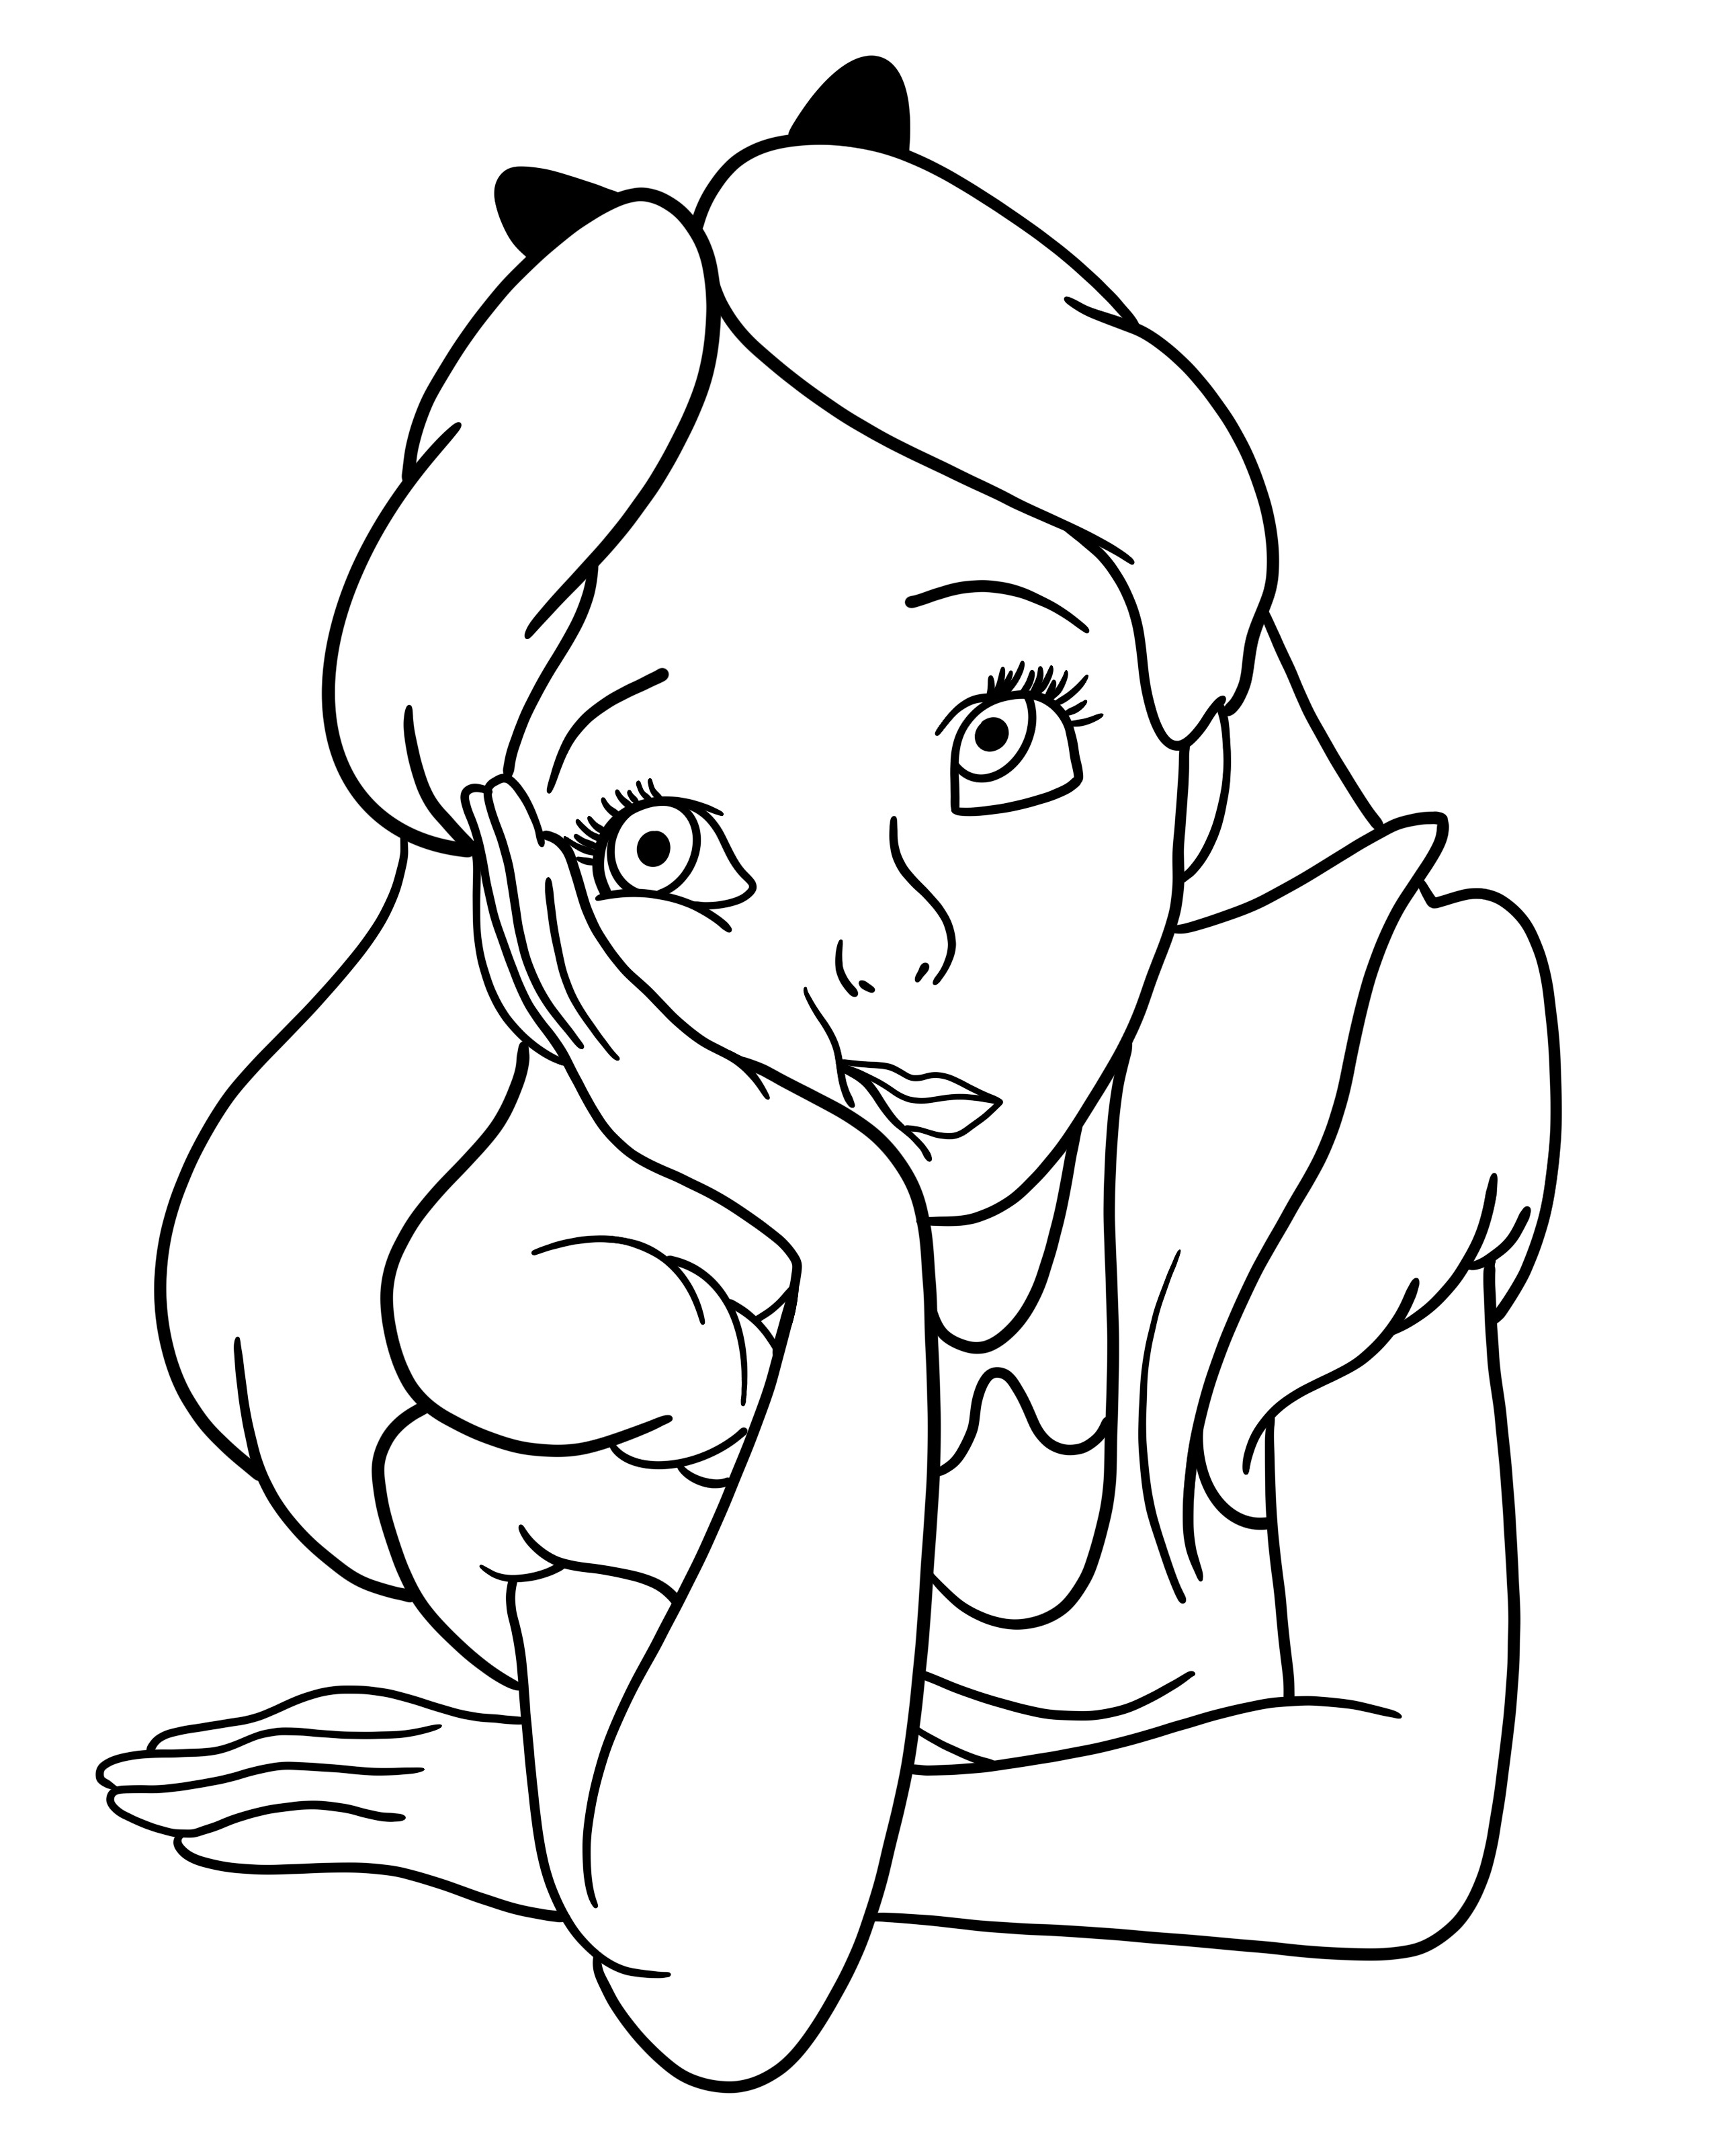
\includegraphics[width=3.0cm]{images/shutterstock_2075221579.jpg}
\vspace{-2em}
\end{wrapfigure}

На этом этапе можно выполнить много интересных упражнений — вы почти мастер в проектировании дифференцируемых моделей! Для начала, используя любой набор данных для классификации изображений, вы можете попробовать реализовать с нуля Vision Transformer, как описано в Разделе \ref{subsec:transformers_image_audio}, следуя \cite{dosovitskiy2020image} для выбора гиперпараметров. Обучение ViT с нуля на небольшом наборе данных довольно сложно \cite{lee2021vision,steiner2021train}, так что будьте готовы к некоторому разочарованию, если у вас нет достаточной вычислительной мощности для рассмотрения наборов данных размером в миллионы. Вы также можете попробовать более простой вариант, такой как модель Mixer, описанная в Разделе \ref{subsec:mha_variants}. Все эти упражнения должны быть относительно простыми. 

\begin{enumerate}
\item Для токенизации изображения вы можете использовать Einops, как в Листинге \ref{code:einops}, или другие стратегии (например, свёртку с большим шагом). Для небольших изображений вы также можете попробовать использовать каждый пиксель в качестве токена.
\item Для позиционных вложений все стратегии, описанные в Разделе \ref{sec:positional_embeddings}, действительны. Самая простая для ViT — это инициализировать матрицу \textit{обучаемых} вложений, но я предлагаю вам поэкспериментировать с синусоидальными и относительными вложениями в качестве практики.
\end{enumerate}

Вы также можете попробовать реализовать небольшую модель типа GPT. В токенизации текстовых данных много тонкостей, которые мы не рассматриваем. Однако репозиторий minGPT\footnote{\url{https://github.com/karpathy/minGPT}} — это фантастическая дидактическая реализация, которую вы можете использовать в качестве отправной точки.
